%----------------------------------------------------------------------------
\chapter{License plate localization}

This chapter discusses the work done on vehicle and number plate detection. The main goal of this section’s algorithm is to localize number plates on input images. I used deep learning-based object detection for this task. I chose object detection over semantic segmentation because multiple license plates on a single image can be possible. Semantic segmentation does pixel-level classification, thus does not help in distinguishing objects of the same class. Object segmentation would hardly constrain the maximum number of things to find in the same type on the image.

Although the main task is number plate detection, I also decided to include vehicle detection. License plates are usually on vehicles that we want to identify. They have properties like type, make and color. If a stolen number plate is identified, we are primarily interested in the vehicle it belongs to. We can also infer additional information (like number plates without vehicles, which are false positives) by doing vehicle detection.

\section{Data}

The following section describes collecting, analyzing, cleaning, and validating the dataset needed for training. An essential aspect of obtaining the data was to cover as many images as possible with labeled license plates. Thousands of photos are necessary to ensure proper data diversity. The aim was to get not only license plate annotations but also vehicle annotations.

\subsection{Sources}

There were not many standalone datasets meeting these requirements. I conducted my research mainly on Kaggle and the Google Dataset Search engine. The most promising sets had only a few hundred labels.

I examined the Common Objects in Context\cite{MS-COCO} (COCO) and the Open Images\cite{OID} (OID) datasets. These are large sets containing 123,287 and roughly 2 million detection images. I assumed that if at least one of them had license plate annotations, the number of these labels would be enough. Of these, OID has a vehicle registration plate class. As the dataset is huge, I used a Python toolkit to download all the 6,867 images containing these items. I also downloaded all the detection annotations in separate CSV files (OID train, validation, test). The total size of all files was 2.352 GB.

\subsection{Pre-processing}

The application is not limited to detecting only cars. It is necessary because the stolen vehicle database and the police data source contain cars, trucks, motorbikes, and other vehicles.

All the annotations of the downloaded images were kept. OID has a hierarchical class structure from which I chose nine classes representing the new vehicle class (car, airplane, helicopter, boat, motorcycle, bus, taxi, truck, ambulance). I discarded the original OID vehicle class because it contained objects challenging to place in other subclasses like surfboards and wheelchairs. A few less essential types were discarded (like aerial vehicles or snowmobiles) to keep the cardinality of the resulting classes equal. Figure \ref{fig:OID_classes} shows all the classes used from the OID Vehicle branch.

\begin{figure}[htb]
 \centerline{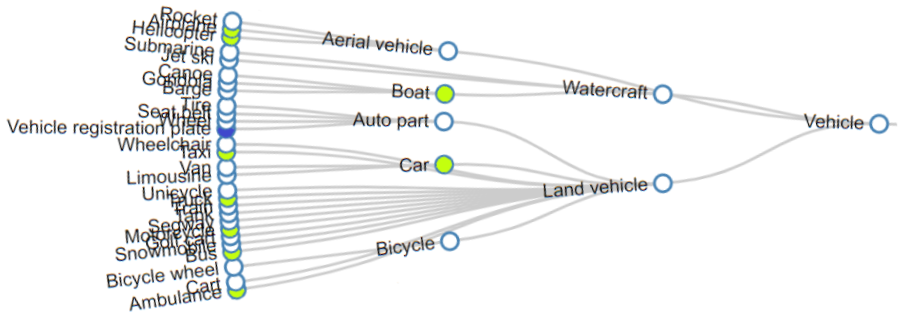
\includegraphics[width=1.0\columnwidth]{.//Figure/PlateLocalization/OID_classes.png}}
 \caption{Selected classes from the original OID Vehicle branch: \textcolor{blue}{license plate}, \textcolor{green}{vehicle}.}
 \label{fig:OID_classes}
\end{figure}

\subsection{Analysis}

I used Power BI to analyze and visualize the downloaded content. My project uses CSV files as data sources. The raw dataset contains 6,867 images with 28,102 bounding boxes, roughly four annotations per image. There are 9,934 vehicle registration plate annotations, one-third of all the boxes. The report revealed that the average image size is $1005\times753$ pixels. While most images have a dimension of $1024\times768$ pixels, some exemptions occur. As the model input is always resized, this is not important to examine more thoroughly.

Table \ref{tab:class_multiplicity} and Figure \ref{fig:class_multiplicity} show that there are more vehicle boxes in the dataset. The left chart shows cardinalities compared to each other, while the right one corresponds to cardinalities relative to the number of images.

\begin{table}[H]
 \caption{Multiplicity of class boxes (left) and the number of images in which a class is present (right).}
 \label{tab:class_multiplicity}
\begin{minipage}{.5\linewidth}
 \centering
\begin{tabular}{ll}
    class & box cardinality\\ \hline
    vehicle & 18,168 \\
    vehicle reg. plate & 9,934 \\
    \textbf{total} & \textbf{28,102} \\
\end{tabular}
\end{minipage}%
\begin{minipage}{.5\linewidth}
 \centering
\begin{tabular}{ll}
    class & image cardinality\\ \hline
    vehicle & 5,806 \\
    vehicle reg. plate & 6,867 \\
    \textbf{total} & \textbf{6,867} \\
\end{tabular}
\end{minipage} 
\end{table}

\begin{figure}[H]
 \centerline{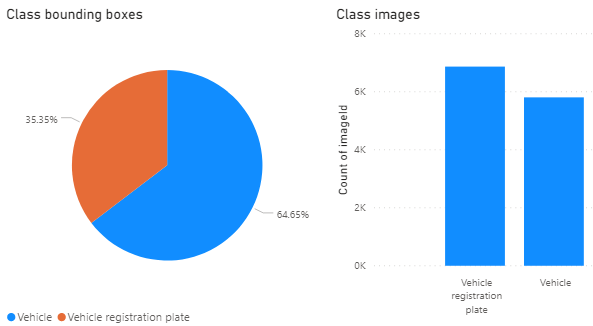
\includegraphics[width=1.0\columnwidth]{.//Figure/PlateLocalization/class_multiplicity.png}}
 \caption{Multiplicity of class boxes and the total number of images per class.}
 \label{fig:class_multiplicity}
\end{figure}

Table \ref{tab:dataset_box_properties} and Figure \ref{fig:median_avg_boxes_plates} show the average bounding box dimensions for license plates. They occupy an average of 10\% of the x-axis and 5\% of the y-axis, which means the detector needs wider anchor boxes of this size. The average number plate box is an elongated rectangle, confirming that the data looks like it should (both vehicles and number plates are usually wider along the x-axis).

\begin{table}[H]
\caption{Dataset box properties.}
\label{tab:dataset_box_properties}
\noindent
\centering
\begin{tabular*}
{\columnwidth}{@{\extracolsep{\stretch{1}}}*{5}{r}@{}}
    type & X\textsubscript{min} & X\textsubscript{max} & Y\textsubscript{min} & Y\textsubscript{max}\\ \hline
    median & $0.41$ & $0.58$ & $0.60$ & $0.68$ \\
    average & $0.44$ & $0.55$ & $0.58$ & $0.65$ \\
\end{tabular*}
\end{table}

\begin{figure}[H]
 \centerline{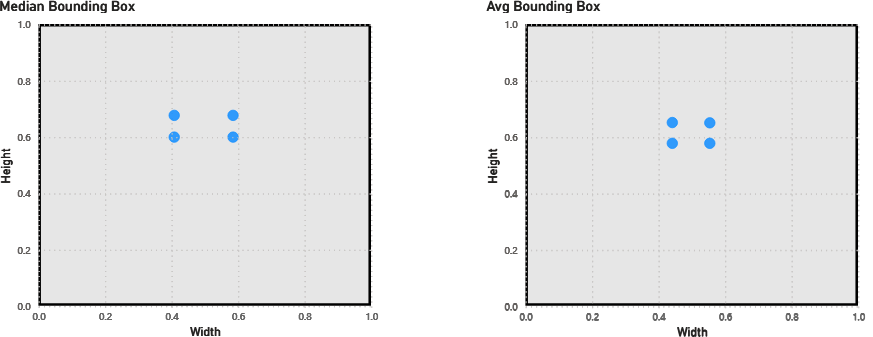
\includegraphics[width=1.0\columnwidth]{.//Figure/PlateLocalization/median_avg_boxes_plates.png}}
 \caption{Median and average bounding boxes of license plates.}
 \label{fig:median_avg_boxes_plates}
\end{figure}

OID has a separate train, validation, and test set. It turned out that they differ in bounding box position distributions, and there is also a slight difference in the average box numbers per image (4.09 vs. 3.33). As the average license plate is also bigger in the validation set, it may be misleading to compare the performance of the models based on that subset. I discovered the phenomenon when I was comparing the average boxes. The phenomenon is illustrated by Tables \ref{tab:avg_boxes_across_subsets} and \ref{tab:median_boxes_across_subsets} and Figure \ref{fig:median_avg_boxes_train_validation}. A closer look confirmed that some outliers did not cause it - the reason was the difference in the distribution of the box sizes across different subsets.

\begin{table}[H]
\caption{Average box coordinates across different subsets.}
\label{tab:avg_boxes_across_subsets}
\noindent
\centering
\begin{tabular*}
{\columnwidth}{@{\extracolsep{\stretch{1}}}*{5}{r}@{}}
    subset & X\textsubscript{min} & X\textsubscript{max} & Y\textsubscript{min} & Y\textsubscript{max}\\ \hline
    $train$ & $0.34$ & $0.65$ & $0.48$ & $0.70$ \\
    $validation$ & $0.21$ & $0.74$ & $0.27$ & $0.65$ \\
\end{tabular*}
\end{table}

\begin{table}[H]
\caption{Median box coordinates across different subsets.}
\label{tab:median_boxes_across_subsets}
\noindent
\centering
\begin{tabular*}
{\columnwidth}{@{\extracolsep{\stretch{1}}}*{5}{r}@{}}
    subset & X\textsubscript{min} & X\textsubscript{max} & Y\textsubscript{min} & Y\textsubscript{max}\\ \hline
    $train$ & $0.38$ & $0.61$ & $0.46$ & $0.66$ \\
    $validation$ & $0.32$ & $0.66$ & $0.32$ & $0.62$ \\
\end{tabular*}
\end{table}

\begin{figure}[H]
 \centerline{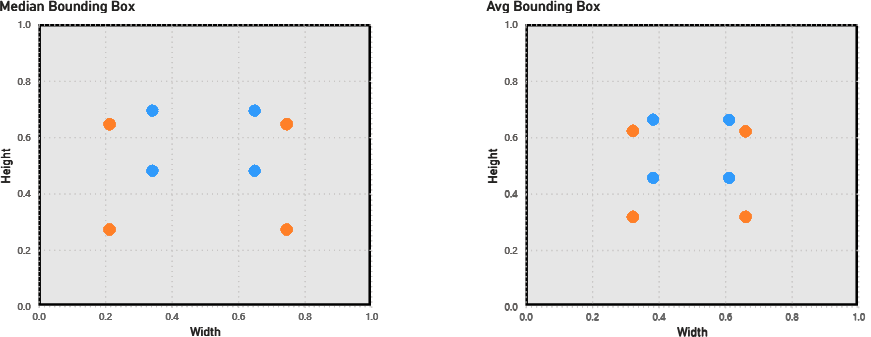
\includegraphics[width=1.0\columnwidth]{.//Figure/PlateLocalization/median_avg_boxes_train_validation.png}}
 \caption{Median and average bounding boxes of \textcolor{blue}{train} and \textcolor{orange}{validation} sets.}
 \label{fig:median_avg_boxes_train_validation}
\end{figure}
\newpage

I applied data aggregation and partition to fix this problem. First, all the images and annotations have been aggregated, then saved to TFRecord\cite{TFRecord} format. It is a binary file format that stores images and custom labels together. This format's main advantage is that it can be processed rapidly, which is not negligible if the dataset has thousands of instances. I created an encoder Python script to generate the dataset files. Detailed contents of such a record are shown below:

\begin{lstlisting}
features {
  feature {
    key: "image/encoded"
    value {
      bytes_list {
        value: binary encoded image
      }
    }
  }
  feature {
    key: "image/height"
    value {
      int64_list {
        value: 769
      }
    }
  }
  ...
  feature {
    key: "image/object/bbox/xmax"
    value {
      float_list {
        value: 0.800000011920929
        value: 0.3006249964237213
      }
    }
  }
  feature {
    key: "image/object/class/text"
    value {
      bytes_list {
        value: "Vehicle"
        value: "Vehicle registration plate"
      }
    }
  }
  ...
}
\end{lstlisting}

The dataset has been evenly sharded between 14 files using Euclidean division \textit{(n \% 14)}. While generating TFRecord batches, I created the corresponding CSV files to analyze later. I selected the validation and test batches, and all the other files became part of the training set. This way, the problem discussed above has been resolved. Table \ref{tab:avg_boxes_after_redistributing} shows the average bounding boxes of the test (12 batches), validation (1 batch), and train (1 batch) sets. They are almost identical.

\begin{table}[htb]
\caption{Average bounding boxes after redistributing the train, validation, and test sets.}
\label{tab:avg_boxes_after_redistributing}
\noindent
\centering
\begin{tabular*}
{\columnwidth}{@{\extracolsep{\stretch{1}}}*{5}{r}@{}}
    subset & X\textsubscript{min} & X\textsubscript{max} & Y\textsubscript{min} & Y\textsubscript{max}\\ \hline
    $train$ & $0.38$ & $0.61$ & $0.45$ & $0.66$ \\
    $validation$ & $0.39$ & $0.61$ & $0.47$ & $0.66$ \\
    $test$ & $0.38$ & $0.60$ & $0.47$ & $0.68$ \\
\end{tabular*}
\end{table}

\subsection{Evaluation}

The final dataset has 5,793 (84\%) training, 537 (7.8\%) validation, and 537 (7.8\%) test images. It has a 23,739 (84\%) training, 2,200 (7.8\%) validation, and 2,163 (7.7\%) test bounding box distribution. There are general dataset division guidelines (like the 70-20-10 rule), from which I deviated. In my opinion, the validation and test sets are already sufficiently representative after reshuffling them in the order of thousands; therefore, I tried to maximize the size of the train set. I created a TFRecord viewer script to validate image and annotation decoding. Figure \ref{fig:training_samples} and \ref{fig:validation_test_samples} show some samples from each subset.

\begin{figure}[H]
 \centerline{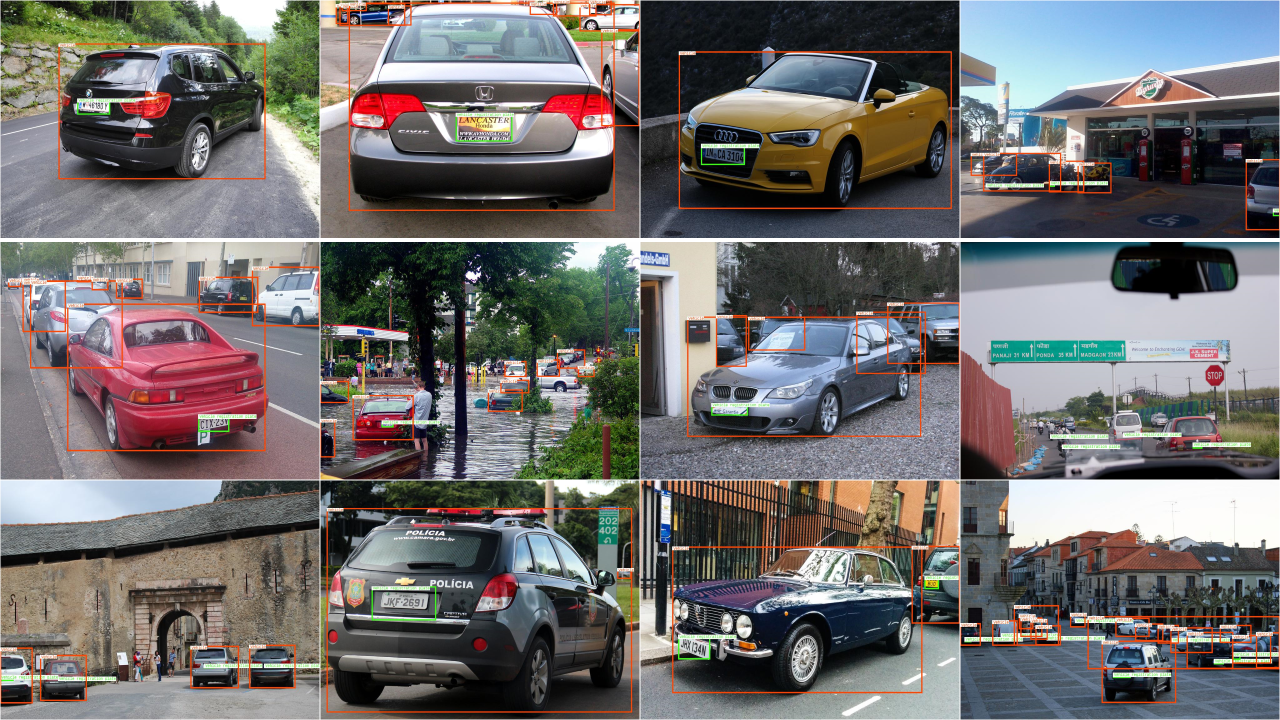
\includegraphics[width=1.0\columnwidth]{.//Figure/PlateLocalization/training_samples.png}}
 \caption{Training samples with bounding boxes: \textcolor{green}{license plate}, \textcolor{orange}{vehicle}.}
 \label{fig:training_samples}
\end{figure}

\begin{figure}[H]
 \centerline{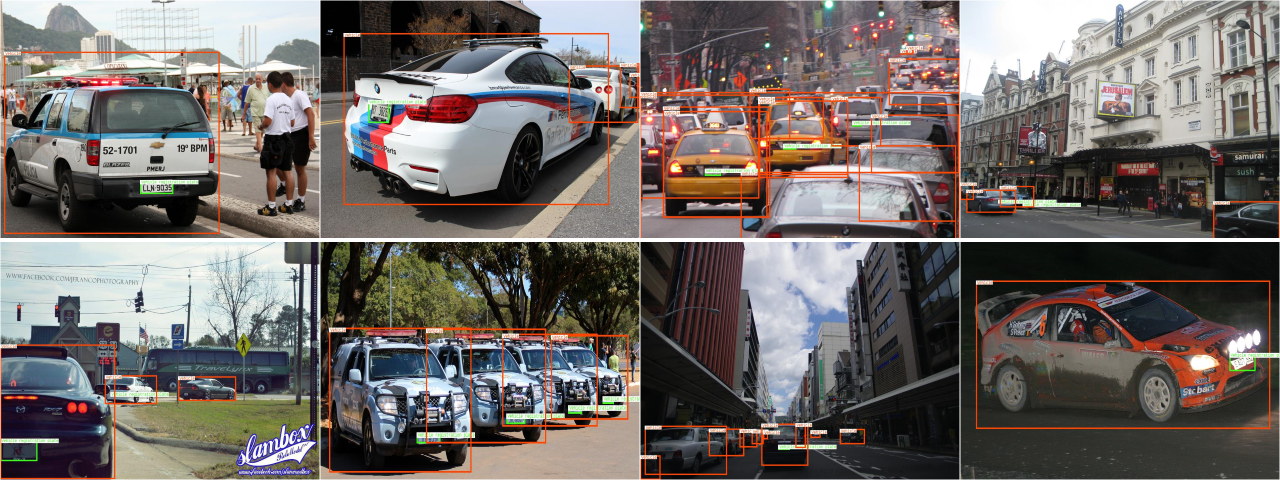
\includegraphics[width=1.0\columnwidth]{.//Figure/PlateLocalization/validation_test_samples.png}}
 \caption{Samples with boxes: \textcolor{green}{license plate}, \textcolor{orange}{vehicle}. 1st row: validation, 2nd row: test samples.}
 \label{fig:validation_test_samples}
\end{figure}

It is important to note that the dataset is not perfect - there are some inconsistencies. It turned out that some images were incompletely annotated. The problems can be categorized in two ways:

\begin{itemize}
  \item Visible license plates are not annotated (Figure \ref{fig:missing_labels} top left).
  \item Vehicle annotations are entirely missing (Figure \ref{fig:missing_labels} top right).
\end{itemize}

One more thing to spot: as a few original OID classes were discarded to keep the new vehicle class close to the cardinality of vehicle registration plates, some types of boxes (like vans) were dropped (bottom row of Figure \ref{fig:missing_labels}). This is partly the reason for some of the missing bounding boxes.

\begin{figure}[htb]
 \centerline{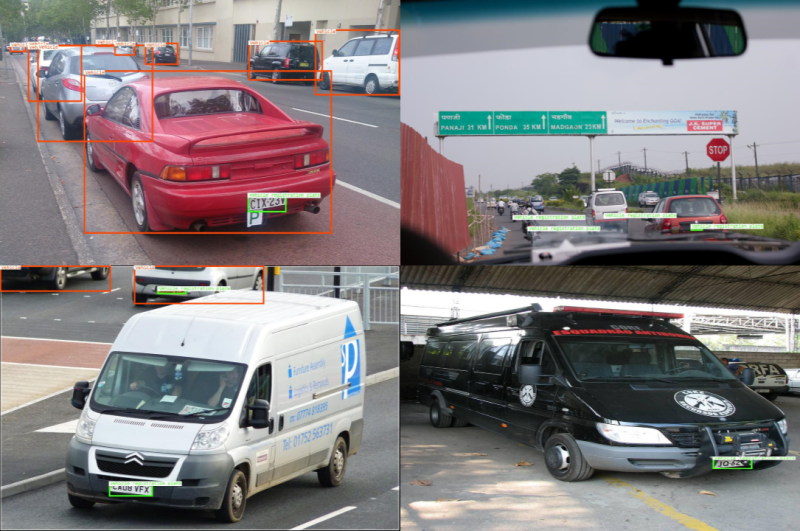
\includegraphics[width=0.8\columnwidth]{.//Figure/PlateLocalization/missing_labels.png}}
 \caption{Top row: inconsistently missing labels. Bottom row: no vehicle boxes around vans.}
 \label{fig:missing_labels}
\end{figure}

These are good examples that while the dataset may be appropriate for the task, it has its flaws. Since balancing classes relative to each other is a priority to avoid bias, I have not made further changes.

\section{Algorithm}

In the following part, I present the preliminary steps of model creation (choosing appropriate metrics), architecture selection, training and fine-tuning, and then post-production (quantization, wrapping).

I chose the COCO evaluation protocol mainly because it measures performance on different-sized objects. As discussed earlier, the vehicle registration plates are relatively small on the images, so I wanted to see how different sizes affect performance. In my opinion, OID would not have been suitable for this task because I would have lost size-specific indicators, but I would not have won with the class-level metrics because there are only two classes.

\subsection{Workflow}

Different data subsets have different roles during the development process. The main idea is to train models on the training set (with most images) and evaluate them on the validation set. When the best model is selected based on its validation performance, it is re-evaluated on an unknown test set to spot if overfitting occurs - which is the case when the model performs noticeably weaker on the new set. Sometimes, this type of overfitting happens as we select the best model based on the validation set – and it remains unnoticed if we do not apply this technique. I used the workflow with the different subsets outlined by Figure \ref{fig:subsets_workflow}.

\begin{figure}[htb]
 \centerline{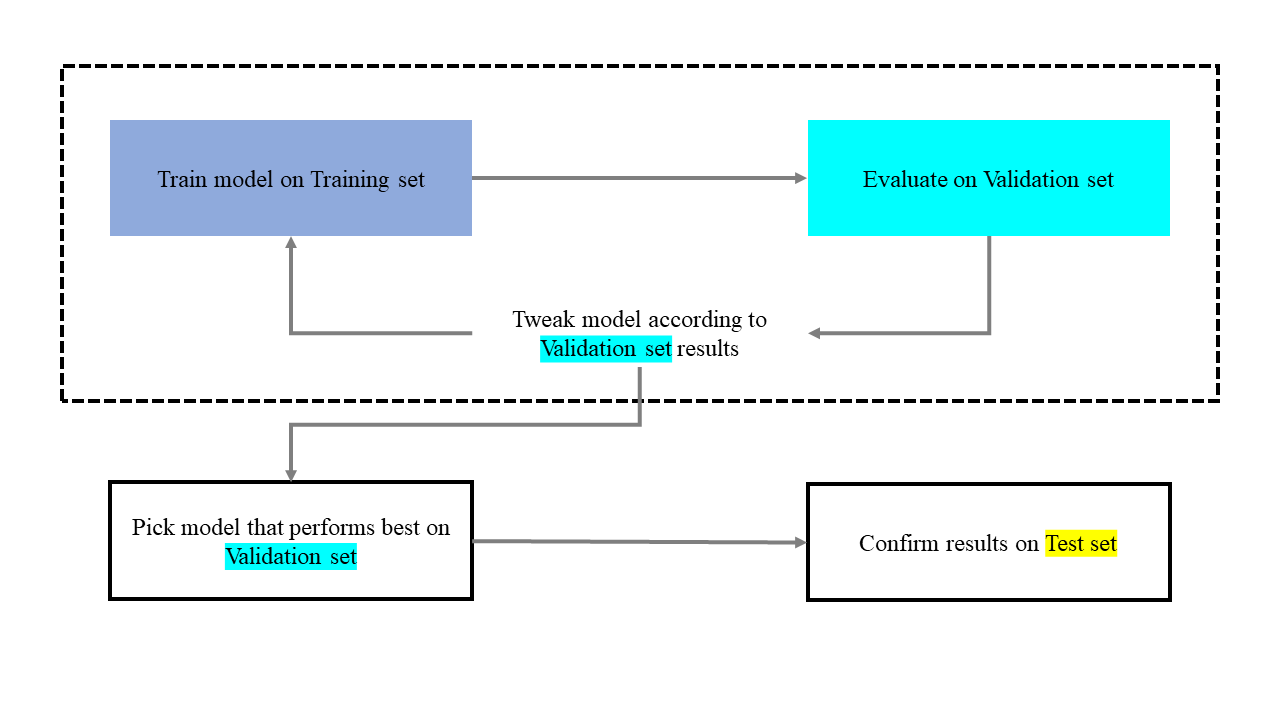
\includegraphics[width=1.0\columnwidth]{.//Figure/PlateLocalization/subsets_workflow.png}}
 \caption{Workflow with different subsets. Source: \cite{ValidationSet}}
 \label{fig:subsets_workflow}
\end{figure}

Training is concluded in a Python/Jupyter environment on a Colaboratory instance. After installing and testing external dependencies, the described steps are applied to each training session. I download base models from TensorFlow's model zoo with or without pre-trained weights (depending on the training configuration). To continue a previous session, I import saved models from Google Drive. The TFRecords are also placed as zip files on Google Drive. They store data on a different server than where the Jupyter instance runs. I download and extract the dataset every time a new session starts (thus, there is no need for network communication during training).

During preprocessing, it is defined how many possible input classes exist. I encode the background as a class (with zero labels to encode non-object image parts as negative examples). I apply fixed shape input image resizing as the dataset has pictures with various resolutions, but the detector expects a static input shape corresponding to the backbone network’s input. The anchor box generator properties are also defined during preprocessing.

In the architecture part, the backbone network and the box predictor are configured separately. I experimented with the classifier and its convolutional hyperparameters (e.g., activation function, regularization, batch normalization). Box predictor properties (like convolutional kernel size or depthwise convolution, batch normalization, activation function) have been tuned similarly.

It is an exciting topic of what loss functions to use in an object detection problem. I use focal loss\cite{TFSigmoidFocalCrossEntropy} for classification and Huber loss (which is very similar to Smooth L1 loss\cite{SmoothL1Loss}) for localization. It is worth mentioning that I started with sigmoid classification loss and online hard example mining (with three negative object samples per one positive) in a way like the original SSD paper\cite{SSD} suggests. However, after researching the topic, I learned about focal loss and RetinaNet\cite{RetinaNet}, using a different approach eliminating foreground-background class imbalance (by down-weighting the loss assigned to well-classified items and by preventing easy negatives from overwhelming the detector during training). Since focal loss takes care of it, hard example mining is unnecessary. Huber loss is used for localization because it handles outliers outside a delta value quite well. Both loss functions contribute equal weight to the total loss.

Post-processing properties, like how many images are allowed on the network’s output after non-maximum suppression, are essential questions to be decided. Since there are potentially many cars and license plates on a street scene, I maximized the network output in 100 detectable objects (although an average image from the dataset has four objects).

Training properties, like batch size, number of steps, variable freezing, optimization algorithm, and the corresponding subsets' path, are defined in the last part of the pipeline. I used four data augmentation techniques (horizontal flip, crop, padding, brightness adjustment) to prevent overfitting. Padding can be interpreted as an out zooming process that reduces bounding box sizes, thus helping one-stage detectors, which are generally poor in localizing small objects. This decision was inspired by the procedure described in the SSD paper\cite{SSD}. Image augmentation samples can be seen in Figure \ref{fig:img_augmentation}. An image and its bounding box coordinates are always augmented with the same transformation. During an evaluation, augmentation is not used to measure performance objectively and ensure that the results are independent of random transformations.

\begin{figure}[htb]
 \centerline{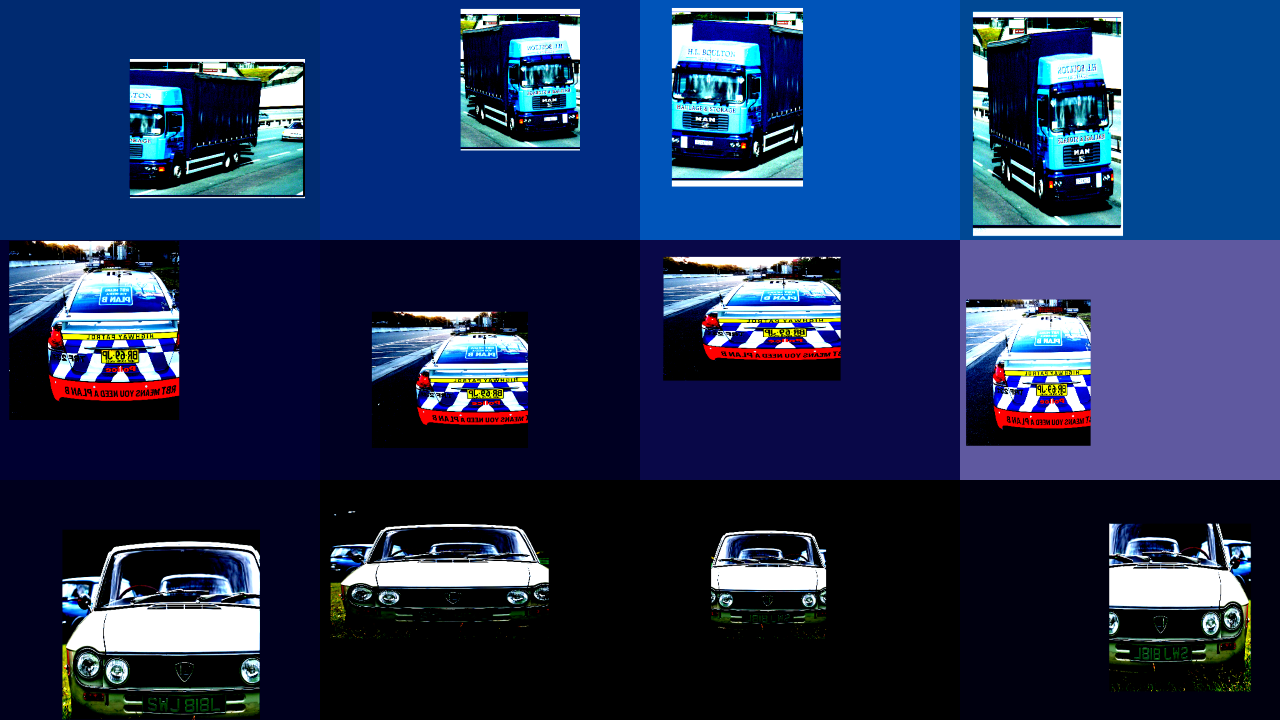
\includegraphics[width=0.8\columnwidth]{.//Figure/PlateLocalization/img_augmentation.png}}
 \caption{Randomly augmented image samples during training. The same transformation is needed for an image and its bounding boxes.}
 \label{fig:img_augmentation}
\end{figure}

\subsection{Optimization}

In this part, I compare the models by summarizing their results in tables. Since multiple values were measured, I only display mAPs. All the trained models' metrics (training duration, mAP, loss) can be viewed in a comprehensive table in the Appendix. For length reasons, I use some abbreviations in the Tables of this section. The metrics \textit{@.50, @.75, small, medium, large} are the mAP values at the corresponding IoU thresholds and object sizes based on the COCO evaluation metrics\cite{MS-COCO}. Model sizes are provided in megabytes. The single numeric value in the input columns is the pixel width and length of the input image. The lr columns stands for learning rate.

Once the input configurations were selected, I started training the models. In the beginning, to save time, I used pre-trained weights (on the COCO 2017 dataset). I kept the same settings of the networks as they were pre-trained. I applied cosine decay learning rate in each case to prevent too optimistic gradient change at the beginning (started from \(\frac{1}{40}\) of the base learning rate, trained like this for \(\frac{1}{20}\) of time, then increased it).

Since training a detector is time-consuming, I drew conclusions based on the results and the learning curve's nature after three epochs (around 17,000 images). One epoch is when the entire dataset is passed forward and backward through the network. The best solution is to apply early stopping (training finishes when model performance permanently stagnates/falls back). However, fewer training sessions would have been possible in this case because there is a minimal improvement over a long period at the end of the flattened learning curve.

I used the same anchor box configuration for all the networks. I used five different-sized grids with a total of 12,804 anchor boxes.

\subsubsection{Architectures}

Generally, a two-stage detector takes a classifier and evaluates it in different locations. Because of the separate steps, these are slower architectures but perform better with various-sized objects. TensorFlow Object Detection API currently supports Faster R-CNN from these variants. Although the inference speed is comparable to one-staged architectures, TFLite conversion is not working – therefore, I solely concentrated on one-stage detectors. SSD, RetinaNet, EfficientDet are supported (YOLO is missing and not likely to be added). Since the detector needs to run on smartphones, choosing a relatively small and fast model was the priority. To start with, I tried 3 different options: RetinaNet (ResNet50), RetinaNet (MobileNetV2), and EfficientDet (EfficientNetD0). I did not try VGG-16 because it is no longer used in modern architectures due to its too many parameters. I used all the networks with the smallest possible input size. Table \ref{tab:starter_architectures} shows the comparison of the starter architectures.

\begin{table}[htb]
\caption{Comparison of the starter architectures.}
\label{tab:starter_architectures}
\noindent
\centering
\begin{tabular*}
{\columnwidth}{@{\extracolsep{\stretch{1}}}*{10}{r}@{}}
    model & size & input & batch & mAP & @.50 & @.75 & small & medium & large\\ \hline
    ResNet50 & 241 & 640 & $8$ & $\textbf{0.389}$ & $\textbf{0.678}$ & $\textbf{0.404}$ & $\textbf{0.116}$ & $\textbf{0.394}$ & $\textbf{0.531}$\\
    EfficientNetD0 & 42 & 512 & $16$ & $0.314$ & $0.581$ & $0.302$ & $0.019$ & $0.321$ & $0.492$\\
    MobileNetV2 & 19 & 320 & $16$ & $0.278$ & $0.504$ & $0.269$ & $0.007$ & $0.248$ & $0.492$\\
\end{tabular*}
\end{table}

I found this comparison problematic as the performance was suspiciously proportional to the input size of the models. It is also important to note that ResNet50 was trained with batch size eight because I had insufficient memory to train it with 16-sized batches. To fix these issues, I switched to EfficientNetD1 and MobileNetV2 640, and the same batch/step values have been applied. Table \ref{tab:starter_architectures_same_input} shows the results.

\begin{table}[htb]
\caption{Comparison of different types with the same input size.}
\label{tab:starter_architectures_same_input}
\noindent
\centering
\begin{tabular*}
{\columnwidth}{@{\extracolsep{\stretch{1}}}*{10}{r}@{}}
    model & size & input & batch & mAP & @.50 & @.75 & small & medium & large\\ \hline
    ResNet50 & 241 & 640 & $8$ & $0.389$ & $\textbf{0.678}$ & $\textbf{0.404}$ & $0.116$ & $0.394$ & $0.531$\\
    EfficientNetD1 & 63 & 640 & $8$ & $\textbf{0.391}$ & $0.671$ & $0.400$ & $\textbf{0.119}$ & $\textbf{0.396}$ & $\textbf{0.548}$\\
    MobileNetV2 & 19 & 640 & $8$ & $0.379$ & $\textbf{0.678}$ & $0.386$ & $0.115$ & $0.386$ & $0.517$\\
\end{tabular*}
\end{table}

This comparison shows more balanced results. Unless ResNet50 is the largest model, its performance is not outstanding anymore; EfficientNet seems to outperform it. MobileNet has modest results; however, it is still close to the benchmark.

As inference speed and model size are critical aspects, ResNet should not be considered. EfficientNet is four times larger than MobileNet: the former runs in 54 ms according to TensorFlow's benchmark, while the latter runs in 39 ms. I measured around 150 ms for EfficientDet and 80 ms for MobileNet on a Samsung Galaxy S10 smartphone running on a CPU with dynamic quantization. Their mAPs are relatively close, so I experimented with both networks before committing to one.

\subsubsection{Batch size}

Batch size is the number of samples propagated through the network at once. Bigger batches allow computational speedups but reduce the ability to generalize. On the other hand, if a model is trained with too small batch sizes (perhaps caused by too sample-specific gradient updates), performance decreases. An ideal range of batch sizes is affected by model parameters and the current dataset.

I trained both networks with different batch sizes. The maximum size I could use was 8 in the case of EfficientNet and 24 for MobileNet. When training with batch size 1, I reduced the learning rate by an order of magnitude (from \({8} \times {10^{-2}}\) to \({8} \times {10^{-3}}\)) to avoid divergence caused by too large gradient updates. Results can be observed in Table \ref{tab:different_batch_sizes}.

\begin{table}[htb]
\caption{Training results with different batch sizes.}
\label{tab:different_batch_sizes}
\noindent
\centering
\begin{tabular*}
{\columnwidth}{@{\extracolsep{\stretch{1}}}*{10}{r}@{}}
    model & size & input & batch & mAP & @.50 & @.75 & small & medium & large\\ \hline
    MobileNetV2 & 19 & 640 & $24$ & $0.386$ & $0.669$ & $0.376$ & $0.108$ & $0.367$ & $0.512$\\
    MobileNetV2 & 19 & 640 & $16$ & $0.372$ & $0.666$ & $0.378$ & $0.101$ & $0.381$ & $0.508$\\
    MobileNetV2 & 19 & 640 & $8$ & $0.379$ & $0.678$ & $0.386$ & $0.115$ & $0.386$ & $0.517$\\
    MobileNetV2 & 19 & 640 & $4$ & $0.377$ & $0.677$ & $0.381$ & $0.116$ & $0.385$ & $0.507$\\
    MobileNetV2 & 19 & 640 & $1$ & $0.261$ & $0.535$ & $0.225$ & $0.090$ & $0.327$ & $0.301$\\
    EfficientNetD1 & 63 & 640 & $8$ & $\textbf{0.391}$ & $0.671$ & $\textbf{0.400}$ & $\textbf{0.119}$ & $0.396$ & $\textbf{0.548}$\\
    EfficientNetD1 & 63 & 640 & $4$ & $0.388$ & $\textbf{0.681}$ & $0.390$ & $\textbf{0.119}$ & $\textbf{0.398}$ & $0.541$\\
    EfficientNetD1 & 63 & 640 & $1$ & $0.291$ & $0.578$ & $0.262$ & $0.100$ & $0.330$ & $0.373$\\
\end{tabular*}
\end{table}

Based on the results, batch sizes 4 and 8 were the most optimal. Both networks produced the most accurate outputs trained with batch size 8. At larger sizes, a decline is observed, especially in detecting small objects. Regarding the other extreme at batch size 1, gradient update per every image seems to confuse the network and reduce its performance. The trend is MobileNet lags by 2-3\% mAP in every configuration behind EfficientNet. On the other hand, MobileNet is four times smaller and significantly faster but slightly less accurate. For these reasons, I decided to use MobileNetV2 for the rest with batch size 8.

\subsubsection{Optimization algorithm and learning rate}

Optimization algorithms\cite{overviewSGD} are used to update network parameters (such as weights) to minimize model loss while training. The most popular method is Stochastic Gradient Descent and its mini-batch variant. This algorithm is relatively easy and powerful, but it usually results in slow convergence. Momentum optimization is generally applied to overcome this issue, introducing and updating gradients' velocity instead of their specific value. Different optimizers exist, such as methods using an adaptive learning rate like RMSprop or Adam.

I tried the Adam, Momentum, and the RMSprop algorithms. Initially, I used the same learning rate \(({8} \times {10^{-2}})\) in all three cases. However, training indicators in the case of Adam and RMSprop showed signs of divergence, so I changed their values to their default learning rate \(({2} \times {10^{-3}})\) based on TensorFlow's optimizer definition. It seems that Momentum's recommended optimum is roughly an order of magnitude larger than what is ideal for the other two. Table \ref{tab:different_opt_algorithms} shows the results.

\begin{table}[htb]
\caption{Comparison of the different optimization algorithms. All the models are MobileNetV2 variants.}
\label{tab:different_opt_algorithms}
\noindent
\centering
\begin{tabular*}
{\columnwidth}{@{\extracolsep{\stretch{1}}}*{9}{r}@{}}
    input & lr & optimizer & mAP & @.50 & @.75 & small & medium & large\\ \hline
    640 & $0.002$ & $Adam$ & $\textbf{0.392}$ & $\textbf{0.682}$ & $\textbf{0.410}$ & $0.103$ & $\textbf{0.412}$ & $0.546$\\
    640 & $0.08$ & $Momentum$ & $0.391$ & $0.671$ & $0.400$ & $\textbf{0.119}$ & $0.396$ & $\textbf{0.548}$\\
    640 & $0.002$ & $RMSprop$ & $0.361$ & $0.643$ & $0.374$ & $0.079$ & $0.394$ & $0.512$\\
    640 & $0.08$ & $RMSprop$ & $0.155$ & $0.333$ & $0.130$ & $0.007$ & $0.154$ & $0.213$\\
    640 & $0.08$ & $Adam$ & $0.011$ & $0.031$ & $0.004$ & $0.000$ & $0.000$ & $0.018$\\
\end{tabular*}
\end{table}

The last two rows of Table \ref{tab:different_opt_algorithms} show the typical cases of too high learning rates. With values closer to their optimums, algorithms could be compared more realistically. Adam and Momentum produced very similar results, while RMSprop could not perform at their level. However, before concluding, the nature of the learning curves is also worth analyzing to see which algorithm has started to converge and which is still improving.

\begin{figure}[htb]
 \centerline{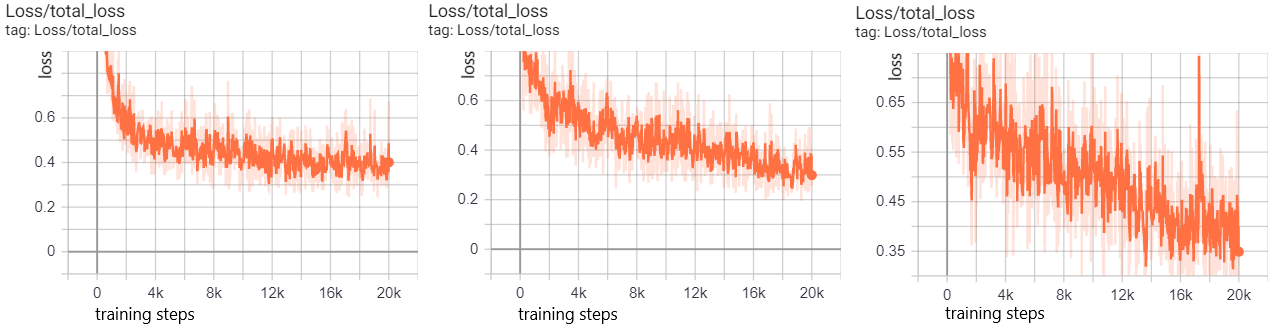
\includegraphics[width=1.0\columnwidth]{.//Figure/PlateLocalization/optimization_algorithm_comparison.png}}
 \caption{Total loss trends of RMSprop (left), Momentum (center), and Adam (right).}
 \label{fig:optimization_algorithm_comparison}
\end{figure}

Figure \ref{fig:optimization_algorithm_comparison} shows that RMSprop not only lags behind but already converges strongly and slightly improves after 14,000 steps. On the other hand, Momentum and Adam still improve. Out of the two, Adam oscillates more, which may sign a too high learning rate. However, the constant improvement after 20,000 steps (and the fact that I use decay learning rate, but oscillation does not decrease) instead suggests that this is more of behavior due to the algorithm's nature, which needs further investigation. Another thing to spot: although Adam performs better in almost everything, Momentum has a significant edge in training detectors to find small objects.

Therefore, I executed another 20,000 steps with the last two algorithms, and I also tried Adam with an order of magnitude lower learning rate \(({2} \times {10^{-4}})\). After this iteration, each case surpassed the optimum and started to overfit. Table \ref{tab:best_optimization_algorithms_comparison} shows the results. It seems that Momentum has the edge: it has improved until reaching 0.393 mAP, while the best of Adam is 0.391, before stagnating around 0.387. The latter could not improve with the lower learning rate, resulting in 0.383 mAP. Thus, the final model to take is the one trained with Momentum.

\begin{table}[htb]
\caption{Comparison of the best results of Momentum and Adam. All three cases indicate the best-performing models before overfitting. All the models are MobileNetV2 variants.}
\label{tab:best_optimization_algorithms_comparison}
\noindent
\centering
\begin{tabular*}
{\columnwidth}{@{\extracolsep{\stretch{1}}}*{10}{r}@{}}
    input & lr & optimizer & mAP & @.50 & @.75 & small & medium & large\\ \hline
    640 & $0.008$ & $Momentum$ & $\textbf{0.393}$ & $\textbf{0.686}$ & $0.391$ & $\textbf{0.119}$ & $0.392$ & $\textbf{0.545}$\\
    640 & $0.002$ & $Adam$ & $0.391$ & $0.685$ & $\textbf{0.404}$ & $0.108$ & $\textbf{0.404}$ & $0.543$\\
    640 & $0.0002$ & $Adam$ & $0.383$ & $0.669$ & $0.380$ & $0.116$ & $0.390$ & $0.528$\\
\end{tabular*}
\end{table}

\subsection{Model deployment}

When the model training is ready, it is time for quantization, TFLite conversion, and to generate the auxiliary structures for deployment.

\subsubsection{TensorFlow Lite conversion and quantization}

During model conversion, it is necessary to note that not all TensorFlow operations are implemented in TFLite. To avoid conversion problems, I checked the compatibility table to see whether the operations in the model (e.g., activation function, depthwise convolution) could be converted. The resulting TensorFlow Lite file at the end of the process can run on Android devices using an interpreter.

\begin{figure}[H]
 \centerline{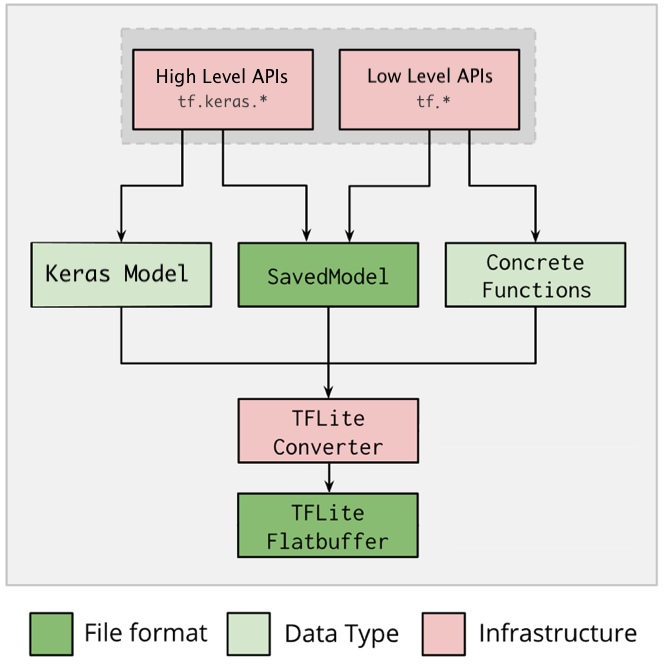
\includegraphics[width=0.5\columnwidth]{.//Figure/PlateLocalization/tflite_converter.png}}
 \caption{TensorFlow Lite conversion process. Source: \cite{TensorFlowLiteConverter}}
 \label{fig:tflite_converter}
\end{figure}

\subsubsection{Input- and output formats}

The detector expects $640\times640$ pixel RGB images on its input. The input is channels\char`_last encoded (order of indices: height, width, red, green, blue). The value of one channel of a pixel is encoded in 8 bits (1 byte). On all three RGB channels, the values are interpreted as 8-bit integer numbers, which must be between 0 and 255.

The model outputs a Hash Map containing four arrays mapped to the indices 0-3. Arrays 0, 1, and 2 describe 100 detected objects, with one element in each array corresponding to each object. There are always 100 detection proposals. A brief description of the arrays is as follows:

\begin{itemize}
  \item \textit{Boxes}: Multidimensional float32 tensor of shape [1, num\char`_boxes, 4] with box locations. Floating-point values are between 0 and 1, the inner arrays representing bounding boxes in the form [top, left, bottom, right].
  \item \textit{Classes}: A float32 tensor of shape [1, num\char`_boxes] with class indices, each indicating the index of a class label from the labels file.
  \item \textit{Scores}: A float32 tensor of shape [1, num\char`_boxes] with class scores. Values between 0 and 1 represent the probability of the detected class.
  \item \textit{Number of boxes}: float32 tensor of size 1 containing the number of detected boxes.
\end{itemize}

\subsubsection{Auxiliary structures}

It is necessary to use an auxiliary structure to interpret the output of the detector. To do this, I created a file containing the names of the output classes in the correct order line by line, including the background class.

The file model\char`_info.txt explains the corresponding model. It contains general information about the network, such as the definition and interpretation of the input and output data formats required for use.

\subsubsection{Summary}

This section dealt with data preparation, architecture selection, training and fine-tuning, and the detector post-production steps. I concluded a total of 184 hours of training with 23 different configurations. The detailed results of the final model can be seen in the table below. Compared to the first initial training from this network family, 1.4\% gain has been reached in COCO mAP. The final detector's size is 35.38 MB, its quantized counterpart is 11.19 MB. Some properties of the selected model are shown in Table \ref{tab:final_model_summary}.

\begin{table}[htb]
\caption{Final model training properties. The architecture is MobileNetV2 trained with the Momentum optimizer (learning rate=\({2} \times {10^{-4}}\), batch size 8).}
\label{tab:final_model_summary}
\noindent
\centering
\small\begin{tabular*}
{\columnwidth}{@{\extracolsep{\stretch{1}}}*{11}{r}@{}}
    input & steps& pre-trained? & duration & mAP & @.50 & @.75 & small & medium & large\\ \hline
    640 & $30,000$ & Yes (COCO) & 8h 50m & $0.393$ & $0.686$ & $0.391$ & $0.119$ & $0.392$ & $0.545$\\
\end{tabular*}
\end{table}